\documentclass{bschlangaul-theorie}
\bLadePakete{cpm,mathe,gantt}

\begin{document}
\let\SZ=\bCpmSpaetI
\let\FZ=\bCpmFruehI
\let\f=\footnotesize
\let\vz=\bCpmVonZu

%%%%%%%%%%%%%%%%%%%%%%%%%%%%%%%%%%%%%%%%%%%%%%%%%%%%%%%%%%%%%%%%%%%%%%%%
% Theorie-Teil
%%%%%%%%%%%%%%%%%%%%%%%%%%%%%%%%%%%%%%%%%%%%%%%%%%%%%%%%%%%%%%%%%%%%%%%%

\chapter{CPM-Netzplantechnik}

\begin{liQuellen}
\item \cite{wiki:netzplantechnik}
\item \cite{wiki:methode-kritischer-pfad}
\end{liQuellen}

\noindent
Die Methode des kritischen Pfades wird auch
\memph{Tätigkeits-Pfeil-Darstellung} oder CPM-Netzplantechnik (von
englisch \memph{critical path method}, CPM)
genannt.\footcite{wiki:methode-kritischer-pfad}

\section{Netzplantechnik, DIN 69900-1}

„Netzplantechnik umfasst \memph{alle Verfahren} zur Analyse,
Beschreibung, Planung, Steuerung und Überwachung von \memph{Abläufen}
auf der \memph{Grundlage der Graphentheorie}, wobei Zeit, Kosten,
Einsatzmittel bzw. Ressourcen berücksichtigt werden können. Ein Netzplan
ist die graphische oder tabellarische Darstellung von Abläufen und deren
Abhängigkeiten“.
\footcite[Seite 14]{sosy:fs:3}

%-----------------------------------------------------------------------
%
%-----------------------------------------------------------------------

\section{Zentrale Begriffe}

Ein \memph{Vorgang} ist eine abgegrenzte Arbeitseinheit mit
\memph{Anfangs- und Endzeit} (vgl. Arbeitspaket im Projektmanagement).
Er besitzt eine \memph{Dauer}.
%
Unter Berücksichtigung der Dauer der einzelnen Vorgänge und unter
Berücksichtigung ihrer Abhängigkeiten wird ermittelt, wann die Vorgänge
stattfinden.
%
In CPM Netzen werden Vorgänge als \memph{Pfeile zwischen Ereignissen}
dargestellt.
\footcite[Seite 15]{sosy:fs:3}

\section{Zweck}

\begin{itemize}
\item Darstellen logischer Zusammenhänge
\item Zeitplan für alle Vorgänge entwickeln
\item Kritischer Pfad und Ressourcen-Engpässe identifizieren
\item Terminüberwachung, laufende Kontrolle
\end{itemize}

\section{Vier Teilaufgaben}

\begin{itemize}
\item Kapazitätsplanung
\item Kostenplanung
\item Strukturplanung
\item Zeitplanung / Zeitfenster
\end{itemize}
\footcite[Seite 22]{sosy:fs:3}

%-----------------------------------------------------------------------
%
%-----------------------------------------------------------------------

\section{Konstruktion eines Netzes}

Dem Vorgang $A_k$ wird ein Pfeil $e_k$ zugeordnet und mit dessen Dauer
bewertet.
%
$i_k$ und $j_k$ sind Anfangs- und Endereignis.
%
Die Anordnung erfolgt nach der Ende-Start-Beziehung.

\begin{center}
\begin{tikzpicture}
\bCpmEreignis[name=i]{$i_k$}{0}{0}
\bCpmEreignis[name=j]{$j_k$}{4}{0}
\bCpmVorgang{i}{j}{$e_k$}
\end{tikzpicture}
\end{center}

\begin{description}

\item[Regel 1:] Folgen die Vorgänge $A_3$ und $A_4$ unmittelbar $A_1$
und $A_2$ so gilt:
\footcite[Seite 24]{sosy:fs:3}

\begin{center}
\begin{tikzpicture}
\bCpmEreignis[name=1]{$i_1$}{0}{2}
\bCpmEreignis[name=2]{$i_2$}{0}{0}

\bCpmEreignis[name=m]{}{2}{1}

\bCpmEreignis[name=3]{$j_3$}{4}{2}
\bCpmEreignis[name=4]{$j_4$}{4}{0}

\bCpmVorgang{1}{m}{$e_1$}
\bCpmVorgang{2}{m}{$e_2$}
\bCpmVorgang{m}{3}{$e_3$}
\bCpmVorgang{m}{4}{$e_4$}
\end{tikzpicture}
\end{center}

\item[Regel 2:] Gibt es zwei Vorgänge (parallele Arbeitspakete) mit
demselben Anfangs- und Endereignis, so wird das Endereignis gesplittet
und ein Scheinvorgang eingeführt:
\footcite[Seite 25]{sosy:fs:3}

\begin{center}
\begin{tikzpicture}
\bCpmEreignis[name=1]{$i_1$}{0}{1}
\bCpmEreignis[name=2]{$j_2$}{4}{2}
\bCpmEreignis[name=3]{$j_3$}{4}{0}

\bCpmVorgang{1}{2}{$e_1$}
\bCpmVorgang{1}{3}{$e_2$}
\bCpmVorgang[schein]{2}{3}{$e_0$}
\end{tikzpicture}
\end{center}

\item[Regel 3:] Folgt der Vorgange $A_4$ unmittelbar $A_1$ und $A_2$ und
folgt $A_5$ unmittelbar $A_1$ , $A_2$ und $A_3$ so wird ein
Scheinvorgang eingeführt:
\footcite[Seite 26]{sosy:fs:3}
\end{description}

\begin{center}
\begin{tikzpicture}
\bCpmEreignis[name=1]{$i_1$}{0}{4}
\bCpmEreignis[name=2]{$i_2$}{0}{2}
\bCpmEreignis[name=3]{$i_3$}{0}{0}

\bCpmEreignis[name=4]{$j_4$}{4}{3}
\bCpmEreignis[name=5]{$j_5$}{4}{0}

\bCpmEreignis[name=m1]{}{2}{3}
\bCpmEreignis[name=m2]{}{2}{0}

\bCpmVorgang{1}{m1}{$e_1$}
\bCpmVorgang{2}{m1}{$e_2$}
\bCpmVorgang{3}{m2}{$e_3$}

\bCpmVorgang{m1}{4}{$e_4$}
\bCpmVorgang{m2}{5}{$e_5$}

\bCpmVorgang[schein]{m1}{m2}{$e_0$}
\end{tikzpicture}
\end{center}

\noindent
Es gibt nur eine Quelle (Projektstart) und eine Senke (Projektende).
Ggf. müssen Scheinvorgänge eingeführt werden, um dies zu erreichen.
%
Kann ein Vorgang $A_2$ bereits begonnen werden, wenn ein Teil des
Vorgangs $A_1$ erledigt ist, so wird $A_1$ gesplittet.\footcite[Seite
27]{sosy:fs:3}

\literatur

\end{document}
